\section{Motivation}
Modern day technology has developed under incredible speed in the recent decade and the computing power growth rate is truly phenomenal and lasting impact can be felt and benefit us in many ways. It is important to realise the worldwide effect on the environment by the increase in consumption of power by these technology advancements.

According to ~\cite{pickavet2008worldwide}, the power consumption growth rates of PCs are about 7.5\% per year. Data Centres and network play a much larger role as they both have power consumption rate of 12\% each. This considerable growth is due to increasing data to be accessed, stored and processed. The constant expansion of energy consumption leads to increase in carbon emissions. \(CO_2\) emissions from ICT (Information and communications technology) are increasing at a rate of 6\% per year, at such rate by 2020 it will account to 12\% of worldwide emissions ~\cite{rong2016optimizing}.

\begin{figure}[ht]
    \centering
    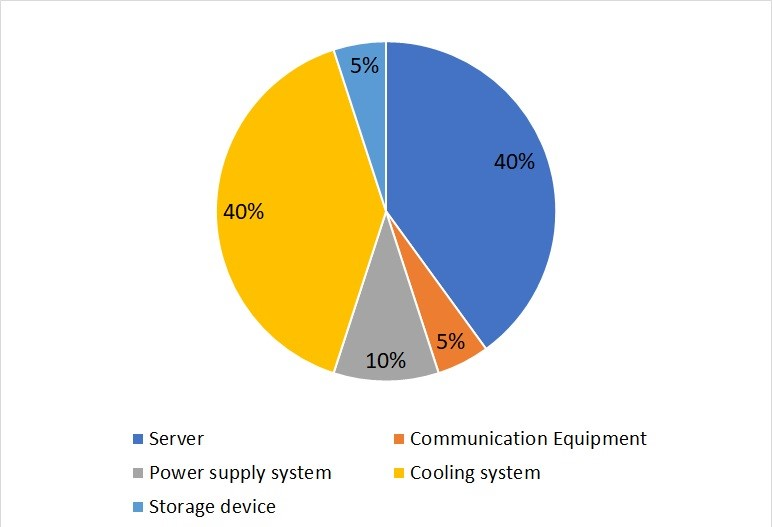
\includegraphics[width=300pt]{energypiechart}
    \caption{\label{fig:energypie} Energy consumption distribution of data centers.}
\end{figure}

The major role of power consumption by a data warehouse is played by the servers and the cooling system which is used to cool down the physical parts of the server. The figure~\ref{fig:energypie}, shows that both the servers and the cooling systems account for 80\% of the total consumption with both accounting for 40\% each~\cite{rong2016optimizing}. Making power and energy one of the key challenges in system and software designs. In order to improve processor's performance while limiting power consumption, designers have increasingly utilized dynamic hardware adaptions. But to guide to these hardware adaptions it is necessary to measure the power of systems accurately. Such adaptations can reduce power consumption and chip temperature by reducing the amount of available performance. Temperature sensors are slow in response due to the thermal inertia of the microprocessor. Relying on them would give slow response and detection of temperature changes. Many demonstrations have been done to show that performance counter/performance events are effective proxies of power measurement \cite{bellosa2000benefits}.

The study of the relations between different performance counters and energy consumption has become crucial. The existence and analysis of the functional relation between them will enable minimization of power consumption leading to less heat generation from the CPU. This decrease in temperature will further reduce the usage of the cooling system. Which all, in turn, leads to cost minimization and a step towards the eco-friendly environment.

Thus, the discovery of the functional relationship between the power consumption and the performance events (PMCs) of the system, will enable the ability to predict the energy consumption for certain computations.

\section{Aims}

The project aims to create a piece of software that will help to understand and find relations between energy consumption and performance counters. The software must aim to be extensible, easy to use and performant. It should be able to perform analysis like regression and clustering on the data. These actions will help in showcasing the relationship of various parameters and the output. The parameters are the performance events and output is the energy consumption by the systems. Following are the objectives that are attempted to be accomplished.

\subsection{Existence of functional relation}

Datasets are mostly in pair of multiple inputs and a single output. And the possibility of the existence of a relation is what has to be found. Is it possible to define the data in a form of function? A question like this is one of the aims. Defining the data in a form of function can be thought of as explaining the dataset in a form of a formula which can combine various parts of the input parameters and match the output. It is quite impossible to tell that whether a function definitely exists. This is because the data is always a subset of the population and there are a number of records which are either not in the dataset or it is not known. But, regardless it can definitely explain the non-existence of a functional relation by finding a pair of input parameters and output that violate the definition of a function.

The pair which violates the definition of a function must be looked at as there is a high probability of that data set record being corrupt or if not it can actually act as a contradiction and explain the non-existence. If this outlier is, in fact, corrupt, this process can be used for data cleanups as well.

\subsection{Analysis of functional relation}

Once, it is not possible to prove functional non-existence in the dataset anymore. The dataset must be analysed in order to better understand the functional relation of the parameters and the output. The analysis of the relation explains the contribution of a parameter to the result. It gives a better understanding of the correlation between two quantities. Does high page faults correlates to high energy consumption? Questions like this are what the analysis tries to answer. This can also be thought of an explanation of the resultant parameter.

In other words, understanding the correlation is the other aim. Once it is known that there is a high correlation. Further investigation can be done in order to find the form of the relation.

\section{Approach}

For each aim, two approaches have been employed. Both the approaches try to achieve the same conclusions but with different methodology.

The experimental data sets provided has the following format:

\(E_1,\ x_{11},\ x_{12},\ x_{13} \ldots x_{1k}\)\\
\(E_1,\ x_{21},\ x_{22},\ x_{23} \ldots x_{2k}\)\\
\ldots \\
\(E_n,\ x_{n1},\ x_{n2},\ x_{n3} \ldots x_{nk}\)

where \(k\) is the number of parameters (performance events), \(n\) is the number of records in the dataset.
\(E_i\) is the experimentally obtained dynamic energy consumption and \(x_{ij}\) are the experimentally obtained performance events (PMCs).

\subsection{Existence of functional relation}

The main objective here is to find the non-existence of functional relationship. In other words, it means proving that the dataset cannot be explained in terms of a function/formula.

First approach here is to find two performance events tuples \((x_{i1},\ x_{i2},\ x_{i3} \ldots x_{ik})\) and \\ \((x_{j1},\ x_{j2},\ x_{j3} \ldots x_{jk})\) that are equal within some tolerance, but their corresponding \(E_i\) and \(E_j\) dynamic energy consumption are different. Existence of such a tuple in database will lead us to prove the non-existence of a functional relationship.

It is, in fact, easier to find two equal records by ordering the dataset by their parameters and going through the entire dataset once to find equal records and comparing their dynamic energy consumption. The order of complexity of such is \(O(N \log(N))\) which is the complexity of sorting as that is the only heavy duty task involved. But it gets complicated when tolerance comes into play. Likewise, the task at hand is to find similar records rather than equal records. The project employs 2 methods to measure the similarity between the two data records.

First approach:

The data records are imagined as data points in \(k-space\) as we have \(k\) number of parameters. Then the whole space is divided into small \(k-dimension\) cubes with dimensions \((t_1, t_2, \ldots t_k)\) where \(t_i\) is the tolerance of each parameter. The data points are then put in their respective cubes. When two points lie in the same cube that means their parameters are similar and so must be there output. If they do not have similar output within some tolerance then they violate the functional relation.

Second approach:

The data points in \(k-space\) are said to be similar if the Euclidean distance between them is less than the \(t\) provided, where \(t\) is the total/max tolerance. In this method, clustering is done using the distance between the parameter vector of the data points.

\subsection{Analysis of functional relation}

Many different types of relations can exist between two variables. But, since the correlation between the variables is known to be linear. Linear regression is done between the dynamic energy consumption with the performance events. Many researchers have been successful in estimating using linear models to estimate energy consumption using performance events.\cite{o2017survey} The preference given to linear models is due to the trickle-down effect of the performance events.\cite{bircher2007complete} Hence, Linear regression is used to analyse the relationship.

Linear regression is done with 2 variables but there are \(k\) variables related to energy consumption making it hard to understand the nature. Multiple linear regression tries to find the best fit to the data but in this process, the best fit hinders the tolerance factor in the dataset and also undermines the actual relation. As multiple regression is also interested in predicting the output variable. Hence to analyse one of the variables, the data point must be grouped using their other \(k-1\) variables. Each grouped cluster is then visited and linear regression is performed. Two approaches are employed to cluster the dataset. These are similar to clustering techniques used in finding the existence of the relation.

First approach:

Data points are clustered by putting the data points in the respective \(k-1\) dimension cube. Forming a cluster with almost similar \(k-1\) variables. Each data point is put in one of the cubes. These data points have similar \(k-1\) performance event vector but varying one of the parameters and output variable. Regression line calculated corresponds to the effect of the parameter variable to the output variable in a particular situation. The situation is the similar \(k-1\) parameter values.

Second approach:

Euclidean distance is used to isolate similar \(k-1\) variables. A \(k-1\) dimension sphere can be imagined for simplicity with its radius being the total/max tolerance. Here, each data point has its own small sphere. The regression line calculated for each data point act as the tangent to the data point in the direction of its neighbours.

\section{Structure of report}

In this report, the motivation behind the project and brief description of the approaches that will be undertaken are seen already.

This Introductory chapter is followed by Background research, design aspects of the software, implementation of the software, testing and evaluation of the tool followed by the conclusion and the future works.

Background research explains about performance events and how do they influence energy consumption by the system. It also explains the approaches in detail mentioned above and analyses their complexity and how they can be optimised.

Following Background research, design and implementation of the software are deep dig into as we want an extensible, performant tool. Testing and evaluation of the software are also explained. How the software is tested and its evaluation of its performance. The report ends with conclusions and future works that shows how the project can be extended and applied to various other domains.